
\title{Multicore MIL}

\author{}

\maketitle

\section{Introduction}
%
We adapt MIL to a multicore setting. MIL programs become threads, but are otherwise to a large extent unchanged from \cite{mil}. Multicopy atomicity: IRIW - if thread 1 sees write by thread 2 then thread 3 sees it as well. Same memory model as in flat \cite{mca-flat}.
%%
%\begin{figure}[t]
%\begin{center}
%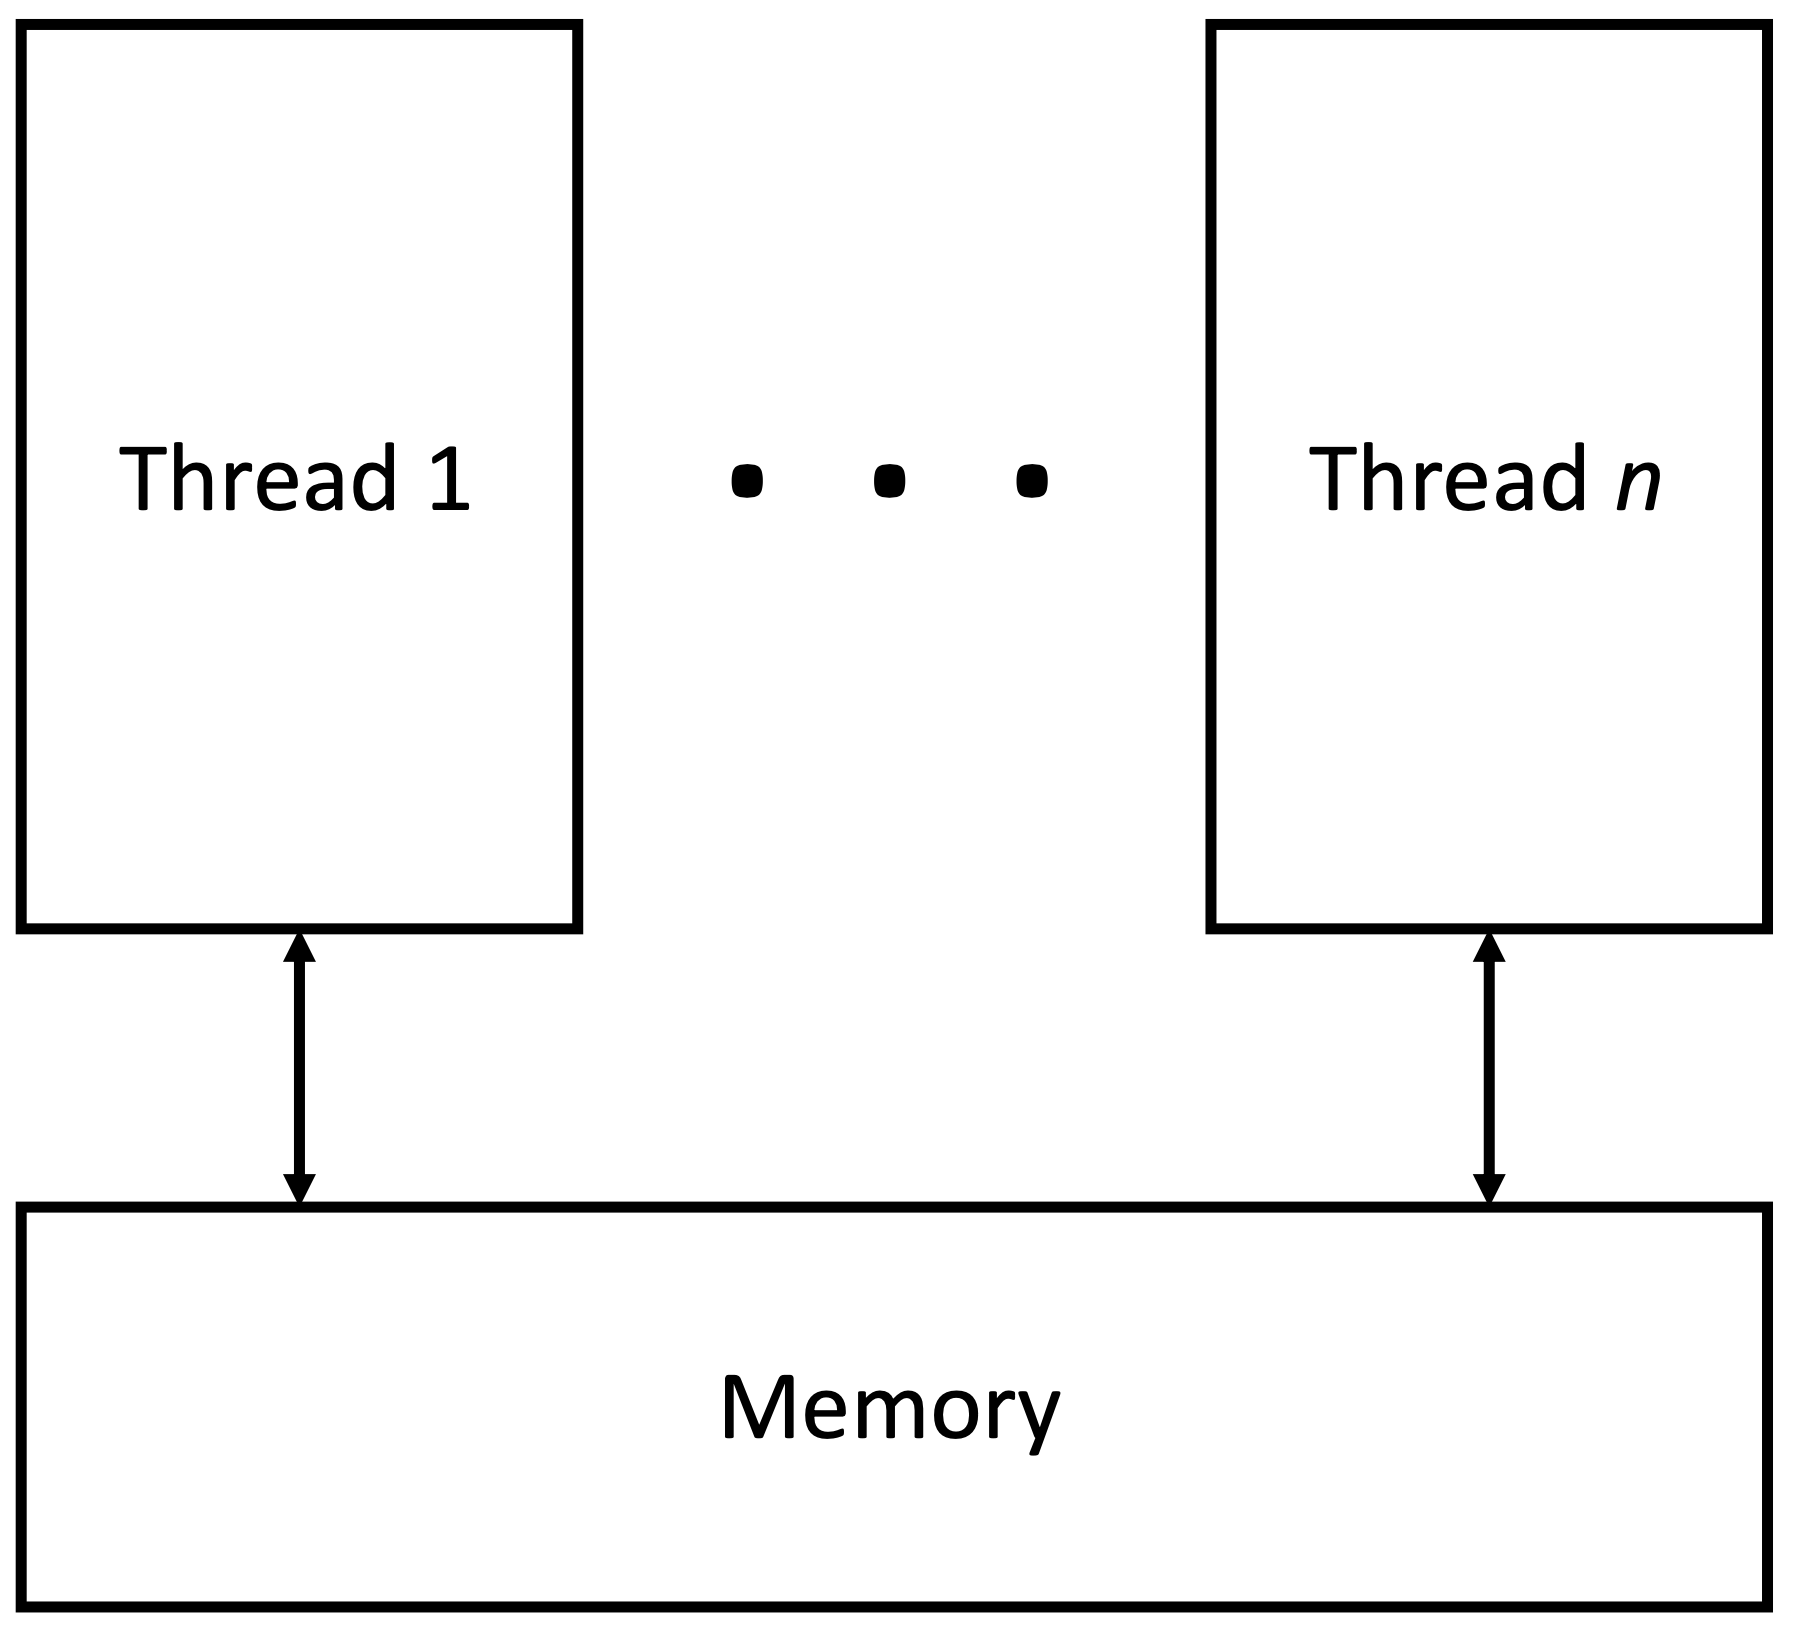
\includegraphics[scale=0.25]{memory.png}
%\end{center}
%\caption{Memory model}
%\label{fig:memory}
%\end{figure}

\section{Programs}
\label{sec:programs}
%
The \MCMIL\ model inherits much of its syntax and basic ideas from (sequential) \MIL\ \cite{MIL}.

\paragraph{Abstract Syntax}
Figure \ref{fig:types} summarizes the abstract syntax of \MCMIL.
%
\begin{figure}
\begin{tabular}{llcl}
%Values & $v\in\Values$ & = & $\Words$ \\
%Addresses & $a\in\Addresses$ & $\subseteq$ & $\Words$ \\
%Registers & $r\in\Regs$ & $\subseteq$ & $\Words$ \\
Names & $m\in\Names$ \\
Thread identifiers & $\tid\in\Tids$ \\
Types & $\type\in\Types$ & ::= & $\pctype\ \mid\ \regtype
%\ \mid \ \memtype
$ \\
Expressions & $\expr\in\Expr$ & ::= & $v\ \mid\ m\ \mid\ \unop(\expr)\ \mid\ \binop(\expr_1,\expr_2)\ \mid\ \cdots$  \\
%Messages & $\msgvar\in \Msg$ & ::= & $\tid:m$ \\
Barriers & $\btype\in\mathit{BTy}$ & ::= & $ \mathit{R}\ \mid\ \mathit{W}$ \\
%Unsourced ops & $\uop\in\UOps$ & ::= & $\expr$ \\
%  & & & $\mid \ \store{\type}{m_a}{m_v}$ \\
%  & & & $\mid\ \acq{\btype}\ \mid\ \rel{\btype}$ \\
%  & & & $\mid\ \cas{m_i}{m_a}{m_o} $ \\
%Sourced ops & $\sop\in\SOps{}$ & ::= & $\loadsrc{\type}{m_a}{\msgvar}$ \\
%  & & & $\mid\ \loadrsrc{\type}{m_a}{\msgvar}$ \\
%  & & & $\mid\ \storecsrc{\type}{m_s}{m_a}{m_v}{\msgvar}$ \\
%Operations & $\op\in\Ops$ & ::= & $\uop\ \mid\ \sop$ \\
Operations & $\op\in\Ops$ & ::= & $\expr$ \\
  & & & $\mid \ \rread{\type}{m_r}$ \\
  & & & $\mid \ \rwrite{\type}{m_r}{m_v}$ \\
  & & & $\mid \ \load{m_a}{\tid}$ \\
  & & & $\mid \ \store{m_a}{m_v}$ \\
  & & & $\mid\ \loadr{m_a}{\tid}$ \\
  & & & $\mid\ \storec{m_s}{m_a}{\tid}$ \\
  & & & $\mid\ \acq{\btype}$ \\
  & & & $\mid\ \rel{\btype}$ \\
  & & & $\mid\ \cas{m_a}{\tid}{m_i}{m_o}{m_p} $ \\
Microinstructions & $\inst \in \Inst$ & ::= & $\ass{m_c}{m}{\op}$
\end{tabular}
\caption{Types, terms and values}
\label{fig:types}
\end{figure}
%
\todo[inline]{In this account, REMEMBER to assign to the $m_s$ when the
source is determined. Fetch to allocate new $m_s$ along with the instruction name AND order $m_s$ before the instr name.}
%
Instruction include arithmetic/logical operations ($\exp$, left open), register read and write ($\rread{}{}$, $\rwrite{}{}{}$), memory load and store ($\load{}{}{}$, $\store{}{}{}$), load-reserved/store-conditional ($\loadr{}{}{}$, $\storec$), acquire-release ($\acq{}$, $\rel{}$), and CAS ($\cas{}{}{}{}{}$).

Programs are represented in single static assignment (SSA) form as a sequence of consecutively named microinstructions $\inst$ of the form $\ass{m_c}{m}{\op}$ where $m$ is the name of $\inst$, $m_c$ names an enabling condition, a microinstruction returning a boolean, and $\op$ is an operation. Operations can be primitive core-local operations $e$, memory or register load/stores, or concurrency control operations, barriers or atomic operations, here CAS. Names are ordered linearly by the program order $<$.

To ease readability, in Fig. \ref{fig:types} names are indexed according to their intended use. Thus, $m_a$ names a microinstruction returning an address. Similarly, $m_v$ is used for value arguments, $m_s$ for status values, and $m_i$, $m_o$, $m_p$, respectively, for the input, output, and prior values in CAS.

Helper function $\theName(\inst)=m$ is the name of $\inst$, $\theCond(\inst)=m_c$ names (the microinstruction computing the output of) an enabling condition, and $\theOp(\inst) = \op$ is the operation. The free names of $\inst=\ass{m_c}{m}{o}$ are the names occurring in $\op$ along with $m_c$, and the bound name of $\inst$ is $m$. For well-formedness we require that any name $m'$ free in a microinstruction named $m$ must be program ordered before $m$, i.e. $m'<m$.
The syntactic dependency relation $\depends$ is the transitive closure of the relation $R$ on microinstruction names, such that $m\ R\ m'$ ($m$ depends on $m'$) if $m'$ occurs freely in the instruction bound to (named by) $m$. Well-formedness ensures that $\depends$ is irreflexive.
As in \MIL\ \cite{MIL}, names in \MCMIL\ have a dual role both as microinstruction identifiers and as names of the internal resource holding the result of microinstruction evaluation.

HER

\paragraph{Threads}
A thread $\thread\in\Threads$ is a structure
$(\tid,\Valuation,\Dec,\Ftch)$ of which the thread name $\tid$ is unique and immutable. In addition:
\begin{enumerate}
\item
$\Valuation$ is a partial valuation map of names to \emph{assignables}, either a value $v$ or a HER.
\item
$\Dec\subseteq\Inst$ is the set of decoded microinstructions.
\item
$\Ftch\subseteq\Names$ is the set of instruction names that have been fetched.
\end{enumerate}
%
For a thread $\thread=(\tid,\Valuation,\Dec,\Ftch)$ we use $\Valuation_\tid$ to refer to $\Valuation$, and similarly for \Dec_\tid$ and $\Ftch_\tid$.
Also, the uniqueness of $\tid$ justifies to use $\tid$ and $\thread$ interchangably, when no confusion arises.

Threads evaluate programs per thread in SSA fashion. Each microinstruction is evaluated at most once, and accordingly a (macro-)instruction is decoded (or extracted from a buffer holding recently decoded instructions) anew whenever it is encountered in the instruction stream.
The elaboration of an instruction $\inst$ to the point where a sufficient number of free names
have been assigned a value in $\Valuation$ enables $\inst$ itself to be evaluated. These names are those that appear freely in $\inst$, but not in a source message. As result, $\Valuation(m)$ and $m$'s source message, if any, becomes defined as well and, once defined, never reassigned.
Note that the instruction named by $m$ is \emph{not} the same as the value of $m$.
Rather, $\Valuation(m)$ is the result of evaluating the instruction named by $m$ in the current state.
Valuations are extended homomorphically to expressions in the usual way. We assume strictness such that if $\Valuation(\expr)\downarrow$ ($\expr$ is defined in $\Valuation$) then $\Valuation(m)\downarrow$ for all $m$ free in $\expr$. 

The set $\Dec$ represents the  microinstructions obtained as output of the (macro-) instruction decoding phase, in varying states of elaboration. As in \cite{MIL} we abstract from the details of this encoding.

HER, hvad med free names?

We say that an instruction $\inst=\ass{m_c}{m}{\op}$ in $\Inst_\tid$ is \emph{ready}, $m\in\Ready_\tid$, if $\inst$ is enabled ($\Val{\tid}{\expr}\neq 0$), all names free in $\inst$ are assigned in $\Valuation_\tid$, and its result remains to be elaborated, $\Val{\tid}{m}\uparrow$. If instead $\Val{\tid}{m}\downarrow$ we say that $\inst$ is \emph{completed}, $m\in\Completed_\tid$.

The effect of a PC store $\store{\pctype}{m_a}{m_v}$ is, similar to other stores, to write $m_v$ to the resource named by $m_a$, in this instance the PC register. Since there is only one such, the address argument is often elided. A completed PC store can be \emph{fetched}, causing the (proper) instruction encoded somehow and pointed to by the PC register value to be fetched and decoded. This causes the thus decoded microinstructions to enter $\Dec_\tid$. The set $\Ftch_\tid$ is the set of (names of) fetches that have been so executed.


\todo[inline]{Push sources below}

The language of microinstructions is mostly straightforward. Except for loads and stores from/to memory, registers, and the PC, all microinstructions operate on names rather than immediates or addresses. Instructions that depend on previously committed data receive as an extra argument a ``source message'' $\msgvar=\tid:m$, a pair of a thread identifier, $\tid$, and an instruction name $m$, namely the thread and instruction that causes the data to be committed. For instance:
\begin{itemize}
\item For a load $\loadsrc{\type}{m_a}{\tid:m}$ or a
load reserved $\loadrsrc{\type}{m_a}{\tid:m}$, $m$ names the instruction executed by tid $\tid$ from which the load reads, either a regular store $\store{\type}{m_a'}{m_v}$ or a store conditional $\storecsrc{\type}{m_s}{m_a'}{m_v}{\msgvar}$ where
$m_a$ and $m_a'$ name identical addresses.
\item For a store conditional, $\storecsrc{\type}{m_s}{m_a}{m_v}{\tid:m}$,
$m$ names a load reserved instruction $\inst = \loadrsrc{\type}{m_a'}{\tid':m'}$ executed by tid $\tid$,
where $m_a$ and $m_a'$ names identical addresses and such that $\inst$ sets the reservation from which the store conditional reads. Note that the store conditional may be successful or unsuccessful, depending on the presence of stores intervening between the reservation and the store conditional.
\end{itemize}

%Other operations in Fig. \ref{fig:types} represent acquire/release barriers ($\acq{\btype}$, $\rel{\btype}$), load reserved/store conditional ($\loadrsrc{\type}{m}{\msgvar}$, $\storecsrc{\type}{m_s}{m_a}{m_v}{\msgvar}$), and atomics (here, cas, $\cas{m_i}{m_a}{m_o}$).

\todo{HER introduce active names}

\HERTIL

\begin{example}
Show how this captures branch dependencies.
\end{example}

\todo[inline]{Next makes sense only after names can receive values.}

For simplicity we assume that all expressions $\expr$ are strict and total such that, if $m$ occurs (freely) in $\expr$ and $m$ is undefined then the value of $\expr$ is undefined as well, and if all names free in $\expr$ are defined then so is the value of $\expr$. Well-formed programs will have the property that $\mbox{$\depends$}\subseteq \mbox{$>$}$, i.e. if $m$ depends on $m'$ then $m'$ is program ordered before $m$.

\todo{Suffice to say at this point that we have some wf constraints that includes the above. May needd to elaborate later.}


\paragraph{Messages, Memory, Global States}
%
Messages $\msgvar\in\Msg$ are ``located'' names: Pairs $\tid:m$ where $m$ names a completed (fully elaborated and enabled) microinstruction in $\inst_\tid$. Since the instruction bound to $m$ is fully determined by $\tid$, we often identify $m$ in the message $\msgvar$ with its associated instruction $\theInst(\msgvar)$. Similarly, the functions $\theName(\msgvar)$, $\theAddress(\msgvar)$, $\theTid(\msgvar)$, $\theType(\msgvar)$ are getters used to extract the name, resp. address, tid and type of message $\msgvar$. Any ambiguity between messages and instructions is resolved by context. The type of a message $\tid:m$ is the type of (the instruction bound to) $m$, either $\exetype$ for instructions that are neither loads nor stores, and $\pctype$, $\regtype$ or $\memtype$ for the rest. 
The set $\Msg_\tid=\{\msgvar\in\Msg \mid \theInst(\msgvar) \in \Dec_\tid\}$ 
is the set of messages that are local to tid $\tid$. Finally, $\theMemStores(A)$ extracts the memory store messages from the set of messages $A\subseteq\Msg$.

An annotated load instruction $\ass{m}{m_c}{\loadsrc{\type}{m_a}{\msgvar}}$ represents a completed load microinstruction that has taken its input
from (``readsfrom'') the message $\msgvar = \tid':m'$, where $\theInst(\msgvar)$ is a completed store instruction in thread $\tid'$. We call $\msgvar$ the \emph{source} of $m$. This is used to define the happens-before relation below.

Memory $\mem$ is represented as a set of messages $\tid:m$ where $m$ names a
store microinstruction in $\tid$. This modelling of memory is what ensures multicopy atomicity: Prior to entering memory a store microinstruction is visible only locally, and when it enters memory it becomes visible to all.
Finally, states are pairs $\state = \langle \thrdpool,\mem \rangle\in\States$ of a thread pool $\thrdpool : \Tids\rightarrow \Threads$ and a memory $\mem\subseteq\Msg$.

\section{Semantics: Happens-before}

The tool used in \MCMIL\ to account for instruction scheduling (reordering) is the happens-before relation $\hb$.

The key idea is familiar: The happens-before relation must ensure that a
load reads from the most recent ready store that the given thread is able to ``see''. For inter-thread loads readyness is not a problem, since, as we shall see, only ready stores will be visible across threads. For intra-thread loads this is, however, not guaranteed, since, if care is not taken, instruction reordering might cause a store to be ready prior to a PO earlier load whose address or enabledness has not yet been determined, and so should not be visible to that load. To address this we introduce an additional order, a per-thread ``may-depend'' relation $m\maydepend m'$ ($m$ may depend on $m'$), capturing potential store-to-load dependencies similar to the $\strmay$ function of \cite{MIL}.

\begin{definition}[May-depend]
Let $\inst$ be a load or a store named $m$ on address $m_a$, and $\inst'$ a store $\ass{m_c'}{m'}{\store{\memtype}{m_a'}{m_v'}}$, both of thread $\tid$ and of identical type. Then $m\maydepend m'$ ($m$ \emph{may depend} on $m'$), if
\begin{enumerate}
\item $m'$ is PO-prior to $m$, $m' < m$, and
\item either $\Val{\tid}{\expr'}$ or $\Val{\tid}{\expr'}\uparrow$, and
\item either
$\Val{\tid}{m_a}=\Val{\tid}{m_a'}$ or $\Val{\tid}{m_a}\uparrow$ or $\Val{\tid}{m_a'}\uparrow$.
\end{enumerate}
\end{definition}

That is, first, a load to a memory address $a$ can never depend on a
store to register $v$; memory, register, and PC addresses are in effect
disjoint. Second, a load may depend on a store if the store is PO-prior to the load, the store's enabling condition is not known to be false and the store address is not known to be different from the load address. 
This allows to define the happens-before relation $\hb$:

\todo{Change o to \op from here and in the beginning}

\begin{definition}[Happens-before]
\label{def:hb}
\mbox{}
\begin{enumerate}
\item Let $\state$ be a state, and let $\msgvar_1=\msg{\tid_1}{m_1}$, $\msgvar_2=\msg{\tid_2}{m_2}$. Let $R_a$ be a relation on $\mem\cup\bigcup\{\Msg_\tid\mid \tid\ \mbox{tid in }\state\}$ such that $\msgvar_1\ R_a\ \msgvar_2$ if
either of the following conditions hold:
\begin{enumerate}
\item $\tid_1 = \tid_2$ and $m_2 \depends m_1$.
\item $\tid_1 = \tid_2$, $m_1$ and $m_2$ are both identically typed stores, and $m_1 < m_2$.
\item $\tid_1=\tid_2$, $m_1$ is a store on address $a$, $m_2$ is an identically typed annotated load on address $a$ with source $\msg{\tid_1}{m_1}$, and
$m_1$ is maximal under $<$ such that $m_2\maydepend m_1$.
\item $\tid_1\neq\tid_2$, $\msgvar_1\in\mem$, $m_1$ is a store on address $a$, and $m_2$ is an identically typed annotated load with source $\msgvar_1$ on address $a$.
\end{enumerate}
\item The state $\state=\langle \thrdpool,\mem\rangle$ is \emph{valid} if the
transitive closure $R_a^+$ of each relation $R_a$ on $\state$ is irreflexive.
\item
For valid states the \emph{happens-before} relation $\hb_\state$, or just $\hb$ when the state $\state$ is understood from the context, is the relation
$\bigcup\{R_a^+\mid a\mbox{ an address}\}$.
\end{enumerate}
\end{definition}

Notes:
\begin{itemize}
\item Condition \ref{def:hb}.1.a ensures that $\hb$ respects per core syntactic dependencies.
\item Condition \ref{def:hb}.1.b enforces in-order store commits.
\item Condition \ref{def:hb}.1.c is the reads-from relation \cite{readsfrom}.
The maximality condition prevents unelaborated same-thread stores from intervening between $m_1$ and $m_2$.
\item Condition \ref{def:hb}.1.d is similar to \ref{def:hb}.1.c except that
it is left to the scheduler to determine which memory store to read. We show below that for reachable states this does not lead to causal circularities (theorem \ref{thm:validityPreservation}).
\item Condition \ref{def:hb}.2 ensures that the happens-before relation is causally well-founded (loop-free) per location. 
\item $\minMsg(A)$ is the set of minimal elements under $\hb$ of $A$.
\end{itemize}
%
Note that load-store and load-load reordering may cause $\hb$ to become reflexive. Picture/example needed here. This
is not a problem, but indicates that the happens-before terminology may be somewhat misleading. Really we are defining \emph{the} dependency relation on completed microinstructions. 

\subsection{Thread Semantics}
\label{sec:ooo:semantics}
%
We next turn to defining the semantics of microinstructions, in particular the central question ``which value will a given load instruction load?''.
We answer this using the happens-before relation in the standard fashion \cite{Lamport-happens-before}: The source of a memory load will be a maximal store prior to the load in the happens-before order. In fact this will apply also to register loads. The key difference is that register stores are never shared. However, the constraints regarding dependency modelling and microinstruction reordering remain the same regardless if the storage is shared or not.

%The set $\sources(\tid,m,A)$ is defined as follows where
%$\msgvar=m:\tid$:
%%
%\begin{eqnarray*}
%\lefteqn{\sources(\msgvar,A)} \\
%& = & \{\msgvar'=\tid':m'\in A \mid \msgvar'\mbox{ is maximal under }
%\hb\mbox{ such that } m'<m, \type_{m'}=\type_m, \\
% & & \Val{\tid'}{m_a'} = \Val{\tid}{m_a}\mbox{, and if }
%\tid = \tid'\mbox{ then }m \maydepend m''\mbox{ implies }m' \maydepend m''\}
%\end{eqnarray*}
%%
%That is, a store $m'$ is a source of $m$ if there are no PO-later stores in $A$

To provide evidence that the definition using happens-before makes sense we
restrict for the remainder of this subsection to the case of a single core $\tid$ and relate
to the \emph{str-may} and \emph{str-act} sets of \cite{inspectre,MIL}. Let
$\ass{m_c}{m}{\load{\type}{m_a}}$ be a given load instruction. Define:
%
\begin{eqnarray*}
\lefteqn{\strmay(\tid,m)} \\
 & = & \{\ass{m_c'}{m'}{\store{\type'}{m_a'}{m_v'}}\mid
\type'=\type\wedge m' < m \wedge (\Val{\tid}{m_c'} \vee \Val{\tid}{m_c'}\uparrow) \wedge \mbox{} \\
 &   & (\Val{\tid}{m_a}=\Val{\tid}{m_a'} \vee \Val{\tid}{m_a}\uparrow \vee
\Val{\tid}{m_a'}\uparrow) \\
\lefteqn{\stract(\tid,m)} \\
 & = & \{\ass{m_c'}{m'}{\store{\type}{m_a'}{m_v'}} \in \strmay(\tid,m)\mid\mbox{} \\
 &   & \neg\exists\ass{m_c''}{m''}{\store{\type}{m_a''}{m_v''}}\in\strmay(\tid,m).m''>m'\wedge \Val{\tid}{m_c''}\wedge \mbox{} \\
 &   & \Val{\tid}{m_a''} \in\{\Val{\tid}{m_a},\Val{\tid}{m_a'}\}
\end{eqnarray*}
%
In \cite{inspectre,MIL}, a load $m$ reads from a store $m'$ if
$\stract(\tid,m)$ is a singleton $\{\inst'\}$ where
$\inst'$ is a ready store. This motivates the following proposition:
%
\begin{proposition}
Let instructions $\inst=\ass{m_c}{m}{\load{\type}{m_a}}$,
$\inst' = \ass{m_c'}{m'}{\store{\type'}{m_a'}{m_v'}}$ be given.
\begin{enumerate}
\item $\inst'\in \strmay(\tid,m,A)$ iff
$m\maydepend m'$.
\item $\stract(\tid,m,A)=\{\inst'\}$, $\Val{\tid}{m'}\downarrow$, and $\Val{\tid}{m_c'}\neq 0$ iff $\inst'$ is maximal such that $\tid:m'\hb \tid:m$.
\end{enumerate}
\end{proposition}
\begin{proof}
1. Trivial.

\noindent 2. If: Suppose $\msgvar'=\tid:m'$ is maximal such that $\tid:m'\hb\tid:m$. Then def. \ref{def:hb}.1.c applies with $m'=m_1$, $m=m_2$, and $\Val{\tid}{m_a'} = \Val{\tid}{m_a} = a$, and $\msgvar'$ the source of $\msgvar$. 
\todo{Abuse of $a$}
Then $\inst'\in\strmay(\tid,m,A)$, whence $m> m'$. Suppose $\inst''=\ass{m_c''}{m''}{\store{\type}{m_a''}{m_v''}}\in\strmay(\tid,m,A)$ such that $m''>m'$, $\Val{\tid}{m_c''}\neq 0$ and $\Val{\tid}{m_a''} =\Val{\tid}{m_a}$. But this contradicts maximality of $m'$, def. \ref{def:hb}.1.c. Hence
$\inst'\in\stract(\tid,m)$. For uniqueness, if $\inst'''\in\stract(\tid,m)$ and
$\inst'\neq\inst'''$ either $m'''< m'$ or $m' < m'''$. In the first case
$\inst'''\notin\stract(\tid,m)$ and in the second case $m_1$ is not maximal.

Only if: 
Suppose $\stract(\tid,m,A) = \{\inst'\}$, $\Val{\tid}{m'}\downarrow$ and $\Val{\tid}{m_c'}\neq 0$. If $\inst'$ is not maximal according to \ref{def:hb}.1.c
then we find $m>m''>m'$ with instruction $\inst''$ such that $m\maydepend m''$.
If $\Val{\tid}{m_a''}=\Val{\tid}{m_a}$ and $\Val{\tid}{m_c''}\neq 0$ then
$\inst'\notin\stract(\tid,m,A)$ and otherwise $\inst''\in\stract(\tid,m,A)$. Either case is a contradiction, completing the proof.
\end{proof}

\medskip

Following \cite{MIL}, but taking into account the nondeterministic nature of
evaluation in a multicore setting, the microinstruction semantics is given in two steps.  The first is a thread-level instruction evaluation relation
$\singlestep{}{}$ taking a thread state $\langle \tid,\inst,\mem\rangle$ consisting of a tid, a ready or completed instruction, and a memory into a resulting value, and
the second is a system level transition relation $\doublestep{}{}$ accounting for thread and memory interaction, and taking system states to system states.

For $\singlestep{}{}$ let $\msgvar_1$ be a store on $a$ and
$\msgvar_2$ a load on $a$ of equal types. Say that $\msgvar_1$ is a \emph{candidate store} for the (unannotated) load $\msgvar_2$ if either
\begin{itemize}
\item $\tid_1=\tid_2=\tid$ and $\theName(\msgvar_1)$ is maximal under $<$ among stores on $a$ in $\mem\cup\Msg_\tid$ such that $m_2\maydepend m_1$, or
\item $\tid_1\neq\tid_2$ and $\theName(\msgvar_1)$ is maximal under $\hb$
among stores in $\mem$ on $a$.
\end{itemize}
Since only memory stores are ever passed to memory, this definition ensures that
register and PC load only ever see stores that are local, i.e. in  $\Msg_\tid$.

The inference rules governing $\singlestep{}{}$ are given in fig. \ref{fig:ThreadTransitions} and the inference rules for $\doublestep{}{}$ in fig. \ref{fig:SystemTransitions}.
%
\begin{figure}
%
\[
\begin{array}{cc}
(\expRule)
&
\begin{array}{c}
\inst = \ass{m_c}{m}{\expr'} \qquad m\in\Ready \\ \hline
\langle \tid,\inst,\mem\rangle\singlestep{}{}
    \tid(\Valuation_\tid[m\mapsto\Val{\tid}{\expr'}])
\end{array}
\end{array}
\]
%
\[
\begin{array}{cc}
(\stoRule)
&
\begin{array}{c}
\inst = \ass{m_c}{m}{\store{\type}{m_a}{m_v}} \qquad
 m\in\Ready \qquad
 \{\mbox{stores }m'\mid m<m'\wedge m'\in\Completed\}=\emptyset 
 \\ \hline
\langle \tid,\inst,\mem\rangle
\singlestep{}{}
\tid(\Valuation_\tid[m\mapsto\Val{\tid}{m_v}])
\end{array}
\end{array}
\]
%
\[
\begin{array}{cc}
(\ldRule)
&
\begin{array}{c}
\inst=\ass{m_c}{m}{\load{\type}{m_a}} \qquad
m\in\Ready \qquad
\tid':m'\mbox{ is a candidate store for }\tid:m \\ \hline
\langle \tid,\inst,\mem\rangle
\singlestep{}{}
\tid(\Inst_\tid\setminus\{\inst\}\cup\{\inst(\tid':m')\},\Valuation_\tid[m\mapsto\Val{\tid}{m'}])
\end{array}
\end{array}
\]
\[
\begin{array}{cc}
(\ftcRule)
&
\begin{array}{c}
\inst= \ass{m_c}{m}{\store{\pctype}{m_a}{m_v}} \qquad
m\in\Completed \qquad
m\notin\Ftch_\tid \\
\{\mbox{PC stores }m'\mid m'<m\wedge m'\in\Completed\}\subseteq \Ftch_\tid
\\ \hline
\langle \tid,\inst,\mem\rangle
\singlestep{}{}
\tid(\Dec_\tid\cup \translate(\Val{\tid}{m_v}, max(\Dec_\tid)),
     \Valuation_\tid[m\mapsto\Val{\tid}{m_v}],
     \Ftch_\tid\cup\{m\})
\end{array}
\end{array}
\]
\[
\begin{array}{cc}
(\dmbRule - revise)
&
\begin{array}{c}
\inst = \ass{m_c}{m}{\dmbsy} \qquad
\theMemStores(\Msg_\tid) = \emptyset \\ \hline
\langle \tid,\inst,\mem\rangle \singlestep{}{}
\langle \tid(\Dec_\tid[m\mapsto 1])\rangle
\end{array}
\end{array}
\]
%
\caption{Thread level transition relation.}
\label{fig:ThreadTransitions}
\end{figure}

% System transitions

\begin{figure}
%
\[
\begin{array}{cc}
(\OpRule)
&
\begin{array}{c}
\inst = \ass{m_c}{m}{o}\in\Dec_\tid \qquad
\langle \tid,\inst,\mem\rangle \singlestep{}{} \langle\tid'\rangle \\ \hline
\langle \tid\parallel\thrdpool,\mem\rangle \doublestep{}{}
\langle \tid'\parallel \thrdpool,\mem\rangle
\end{array}
\end{array}
\]
%
\[
\begin{array}{cc}
(\ShareRule)
&
\begin{array}{c}
\msgvar \in \minMsg(\Msg_\tid) \qquad \isMemStore(\msgvar)  \\ \hline
\langle \tid\parallel\thrdpool,\mem\rangle \doublestep{}{}
\langle \tid[\Inst_\tid\mapsto\Inst_\tid\setminus\{\msgvar\}]\parallel\thrdpool,\mem\cup\{\msgvar\}\rangle
\end{array}
\end{array}
\]
\caption{System level transition relation.}
\label{fig:SystemTransitions}
\end{figure}
%
The rule $\OpRule$ is restricted to operations that are neither memory stores nor barriers.
 The rule $\ShareRule$ uses the auxiliary predicate $\isMemStore(\msgvar)$ to hold if $\theInst(\msgvar)$ is a memory store. Similarly
$\isRegStore(\msgvar)$ ($\isPCStore(\msgvar)$) holds if $\theName(\msgvar)$ is a register (PC) store.

Comments on the rules:
%
\begin{enumerate}
\item Explain notation
\item Execution steps and bookkeeping steps. Lack of pc
\item Explain \emph{translate}
\item Simple propositions, like monotonicity of the store, downwards closure of $\Inst_{\tid}\cup\mem$.
\item Simplifying assumptions (value domain undetermined, there is always instruction to load, every value is decoded into an instruction)
\item Only local register and PC loads
\item No difference between register and PC loads
\item Programs use only non-annotated loads. Thus annotated loads are never evaluated.
\item In $\ldRule$, $\tid=\tid'$ (proof by invariant)
\item Registers and PC
\item Explain $\ftcRule$
\item Explain $\ShareRule$: Different from the MIL commit. Here a message
can spontaneously decide to migrate from thread local storage (the ``store buffer'') to shared memory.
\end{enumerate}

%
\begin{definition}[Initial state]
An initial state is any state $\state_0 = \langle \thrdpool,\mem\rangle$ such that:
\begin{enumerate}
\item $\Dec_\tid=\{\ass{\top}{m_0}{\store{\pctype}{}{m_v}} \}$ where $m_v$ encodes the first instruction to be executed by thread $\tid$, $\Valuation_\tid = \bot$, and $\Ftch = \emptyset$.
\item $\mem = \emptyset$.
\end{enumerate}
\end{definition}
%

\begin{proposition}
\label{prop:storeMonotonicity}
Let $\state\doublestep{}{}\state'$. Then:
\begin{enumerate}
\item $\mem_{\state}\subseteq\mem_{\state'}$.
\item For all $\tid$, $\mem\cup\Msg_\state(\tid)\subseteq\mem'\cup\Msg_{\state'}(\tid)$.
\end{enumerate}
\end{proposition}
\begin{proof}
1. Instructions never leave memory. 2. Instructions leave $\Msg_{\state}(\tid)$ only when passed to memory. 
\end{proof}

\begin{proposition}
\label{prop: downwardsClosure}
Let $\state$ be a reachable. Then $\Inst_{\tid}\cup\mem$ is $<$-closed.
\end{proposition}
\begin{proof}
Instructions enter $\Inst_\tid\cup\mem$ only when fetched and never leave, by 1. Since they enter in order, the proposition follows.
\end{proof}


\section{Preservation of Validity}

\todo{Haven't checked carefully for notation consistency}

It is trivial to exhibit an invalid state, see fig. \ref{fig:invalid}. For this reason we  restrict attention to reachable states. For this we show that
validity is preserved under transition. Since the initial state is valid, this is sufficent to show validity of any reachable state.

Note that each transition directly affects exactly one thread.
We refer to a transition justified by \OpRule\ in conjunction with one of \expRule, \stoRule, \ldRule\ as an \emph{execution step}.
Say that a transition $\state\rightarrow\state'$ \emph{introduces the message} $\msg{\tid}{m}$, if the transition is by thread $\tid$, and $m$ names the executed instruction. Only execution steps introduce messages and introduced messages are unique. Moreover if no message is introduced in the transition $\state\rightarrow\state'$ then $\hb_\state = \hb_{state'}$.

We get a number of pretty straightforward properties:

\begin{proposition}
\label{prop:introducing}
If $\state=\langle\thrdpool,\mem\rangle\rightarrow\state'=\langle\thrdpool',\mem'\rangle$ then either $\mem'=\mem$ or $\mem'= \mem\cup \{\msg{\tid}{m}\}$ where
$m$ is the name introduced by the transition $\state\rightarrow\state'$ and $\mem'=\mem$. \hfill $\Box$
\end{proposition}

\begin{corollary}
\label{cor:monotonicity}
If $\state=\langle\thrdpool,\mem\rangle\rightarrow\state'=\langle\thrdpool',\mem'\rangle$ then $\mem\subseteq\mem'$ and $\Msg(\tid)\subseteq\Msg'(\tid)$.
\end{corollary}

\begin{proposition}
\label{prop:depends}
Suppose that $\state=\langle\thrdpool,\mem\rangle\rightarrow\state'=\langle\thrdpool',\mem'\rangle$ introduces the message $\msg{\tid}{m_2}$. Then
$m_1\not\depends m_2$ for any message  $\msg{\tid}{m_1}\in\mem\cup\Msg(\tid)$.
\end{proposition}
\begin{proof}
Pick $\msg{\tid}{m_1}\in\mem$. If $m_1\depends m_2$ the instruction
binding $m_1$ has a free name. Then $m_1$ is not in the initial memory, and it is not added in an execution step. The conclusion follows.
\end{proof}

\begin{proposition}
\label{prop:traceback}
Suppose $\state_0\rightarrow \cdots \rightarrow \state_n$,
$\state_0$ is initial, and $\msg{\tid'}{m'}\in\mem_n\cup\Msg_n(\tid)$. Then
there is some $m:0\leq m < n$ such that $\state_0\rightarrow\cdots \rightarrow \state_m$ and  $\msg{\tid'}{m'}$ is the message introduced by the
transition $\state_m\rightarrow\state_{m+1}$.
\end{proposition}
\begin{proof}
By induction on $n$. The base case $n=0$ is trivial. Let $n=n'+1$. By prop. \ref{prop:introducing}, either $\msg{\tid'}{m'}$ is the message introduced by the
transition $\state_{n'}\rightarrow \state_n$ in which case we are done,
or $\msg{\tid'}{m'}\in\mem_{n'}\cup\Msg{\tid}_{n'}$. But then by the IH and
corollary \ref{cor:monotonicity} we find the $m$ meeting the requirements of the induction step.
\end{proof}

Note: need the below for both memory and registers/PC (?)

\begin{theorem}
\label{thm:validityPreservation}
Suppose that $\state$ is reachable, that $\state\rightarrow \state'$ and $\state$ is valid. Then $\state'$ is valid.
\end{theorem}
\begin{proof}
(Sketch)
If state validity is not invariant then we find a transition
$\state\rightarrow \state'$ for which $\state$ is reachable, $\hb_{\state}$ is irreflexive (loop-free) and $\hb_{\state'}$ is not.
By the latter assumption we find a minimal $\hb_{\state'}$-chain
\begin{equation}
\label{eq:chain}
\msg{\tid}{m} = \msg{\tid_0}{m_0}\hb_{\state'}\cdots \hb_{\state'}\msg{\tid_n}{m_n} = \msg{\tid}{m}
\end{equation}
in $\mem_n\cup\bigcup\{\Msg_n(\tid)\mid \tid\mbox{ tid in }\state'\}$.
By prop. \ref{prop:traceback} and reachability of $\state'$ we can assume that $\msg{\tid_i}{m_i}$, $0 < i < n$, is the message introduced by a transition
$\state_{i,2}\rightarrow \state_{i+1,1}$ such that there is an execution
$\pi = \state_0\rightarrow^* \state\rightarrow\state'$ that can be written as
\begin{equation}
\label{eq:chaincomp}
\state_0\rightarrow^*\state_{1,2}\rightarrow\state_{2,1}\rightarrow^*\state_{2,2}\rightarrow\state_{3,1}\rightarrow^* \cdots \rightarrow^*\state_{n-1,2}\rightarrow \state_{n,1}\rightarrow^*\state_{n,2}.
\end{equation}
Note that we cannot in general guarantee
a transition $\state_{0,2}\rightarrow\state_{1,1}$ prior to $\state_{1,2}$ in $\pi$ introducing $\msg{\tid_0}{m_0}$, only that $\msg{\tid}{m}\hb_{\state_{1,2}}\msg{\tid_1}{m_1}$.

In effect, to prevent the chain (\ref{eq:chain}) from existing we must show thatno execution (\ref{eq:chaincomp}) can exist. Intuitively, this is tantamount to showing that aan instruction producing $\msg{\tid_0}{m_0}$ cannot be reordered to the end of the hb chain (\ref{eq:chain}). We can assume that $\msg{\tid}{m}\hb_{\state_{1,2}}\msg{\tid_1}{m_1}$ due to one of def. \ref{def:hb}.1.a--\ref{def:hb}.1.d. In the first case, $m_1\depends m$, which makes it impossible for
$\tid_n$ to produce $\tid:m$ as the last message of. (\ref{eq:chaincomp})
In the second case, $\msg{\tid}{m}\hb\msg{tid_1}{m_1}$ because both $m$ and
$m_1$ are stores and $\tid=\tid_1$. But then, again, it is not possible for
$\tid$ to produce $\tid:m_1$ as the last message of (\ref{eq:chaincomp}).
We can thus conclude that $\msg{\tid}{m}$ is a store to address $a$
and $\msg{\tid_1}{m_1}$ an annotated load with source $\msg{\tid}{m}$ on address $a$. If (case three) $\tid=\tid_1$, $m<m_1$, and again $\msg{\tid}{m}$ cannot be produced as the final message of (\ref{eq:chaincomp}), since then $m_1$ would have to be strictly smaller than $m$, which is a contradiction.
As the final case we obtain that $\msg{\tid}{m}$ is a store on $a$, $\msg{\tid_1}{m_1}$ is a load on $a$ with source $\tid_n:m_n=\tid:m$, and $\tid\neq\tid_1$. Since $\tid_n=\tid \neq \tid_1$ there must exist some $j_0$ such that $\msg{\tid_{j_0+1}}{m_{j_0+1}}$ is a load on $a$ with source $\msg{\tid_{j_0}}{m_{j_0}}$ a store on $a$, and $\tid_{j_0+1}=\tid$, since this is the only way the chain (\ref{eq:chain}) can ``return'' to $\tid$, which it must. But if $\msg{\tid_1}{m_1}$ read from $\msg{\tid_n}{m_n}$ then later in (\ref{eq:chaincomp}), $\msg{\tid}{m_{j_0+1}}$ must have read from a message later than or equal to $\msg{\tid_n}{m_n}$, which it did not. This concludes the argument.
\end{proof}
%
\section{A Promising Semantics for \MCMIL}

We next equip \MCMIL\ with a promising semantics in the style of
\cite{PulteEtAlPromising19}. First some basic def's:
\begin{itemize}
\item $\Timestamps = \Nat$ (timestamps)
\item $\Views = \Timestamps$ (views)
\end{itemize}

\todo{From now on using $d_a$ for addresses and $d_v$ for values}

Thread states $\ts$:
\begin{itemize}
\item $\pc:\PCs$
\item $\pCtl:\PCs\rightarrow \Inst\ \mathit{list}$
\item $\Promises: \Timestamps\ \mbox{set}$: Set of timestamps
\item $\pValuation:\Names\rightarrow \Values\times\Views$
\item $\pRegMap$: $\Regs \rightarrow \Values \times \Views$
\item $\coh$: $\Addresses \rightarrow \Views$ (Timestamps)
\item $\Vrold,\Vwold,\Vrnew,\Vwnew,\Vcap, \Vrel:\Views$
\item $\fwdb: \Addresses \rightarrow \Timestamps \times \Views \times \Bool$
\item $\xclb: \TimeStamps \times \Views\ \mbox{option}$
\end{itemize}

Memory:
\begin{itemize}
\item $\pMsg: \Addresses\times\Values\times\Tids$
\item $\pMem: \pMsg\ \mathit{list}$
\end{itemize}

Expression semantics:
\begin{itemize}
\item $\Sem{v}{\pValuation} = v@0$
\item $\Sem{m}{\pValuation} = \pValuation(m)$
\item If $\Sem{\expr}{\pValuation} = v@\View$ then $\Sem{\unop(\expr)}{\pValuation} = \unop(d)@\View$
\item If $\Sem{\expr_1}{\pValuation} = v_1@\View_1$ and $\Sem{\expr_2}{\pValuation} = v_2@\View_2$ then $\Sem{\binop(\expr_1,\expr_2)}{\pValuation} = \binop(v_1,v_2)@\View_1\sqcup\View_2$
\end{itemize}

Thread semantics in fig. \ref{fig:PromisingThreadTransitions} and assumes a slightly simplified notation where conditions are given as names only.  

\begin{figure}
%
\[
\begin{array}{cc}
(\pExpRule)
&
\begin{array}{c}
\ts.\pValuation(m_c)=d_c@\View_c \qquad d_c \neq 0 \qquad
\Sem{\expr}{\ts.\pValuation}=d_e@\View_e \qquad
\ts'.\pValuation(m) = d_e@(\View_c\sqcup\View_e)
\\ \hline
\langle \tid,t,\ass{m_c}{m}{\expr},\ts,\mem\rangle
\singlestep{}{}
\langle \tid,\ts'\rangle
\end{array}
\end{array}
\]
%
\[
\begin{array}{cc}
(\pStoMemRule)
&
\begin{array}{c}
\ts.\pValuation(m_c) = d_c@\View_c \qquad
d_c\neq 0 \qquad \ts.\pValuation(m_a) = d_a@\View_a \qquad
\ts.\pValuation(m_v) = d_v@\View_v \\
t\in \Promises \qquad \pMem(t) = \langle d_a:=d_v\rangle_\tid \qquad
\Vpre\sqcup\coh(d_a) < t \\
\Vpre = \View_a\sqcup \View_v \sqcup \View_c \sqcup \Vwnew\sqcup \Vcap \qquad
\Vpost = t \\
\ts'.\Promises = \ts.\Promises\setminus\{t\} \qquad
\ts'.\coh(l) = \ts.\coh(l)\sqcup \Vpost \\
\ts'.\Vwold = \ts.\Vwold\sqcup \Vpost \qquad
\ts'.\Vcap = \ts.\coh(d_a) \sqcup\Vpost \\
\ts'.\fwdb(d_a) = \langle t,\Vaddr \sqcup\Vdata,\false\rangle \\ \hline
\langle \tid,\ass{m_c}{m}{\store{\memtype}{m_a}{m_v}},\ts,\pMem\rangle
\singlestep{}{}
\langle\tid,\ts'\rangle
\end{array}
\end{array}
\]
%
\[
\begin{array}{cc}
(\pStoRegRule)
&
\begin{array}{c}
\ts.\pValuation(m_c) = d_c@\View_c \qquad d_c \neq 0 \qquad
\ts.\pValuation(m_a) = d_a@\View_a \qquad \ts.\pValuation(m_v)  = d_v@\View_v \\
\ts'.\pValuation = \ts.\pValuation[m\mapsto d_v @ \View_c\sqcup\View_a\sqcup\View_v] \qquad
\ts'.\pRegMap = \ts.\pRegMap[d_a \mapsto d_v @ \View_c\sqcup\View_a\sqcup\View_v]
\\ \hline
\langle \tid,\ass{m_c}{m}{\store{\regtype}{m_a}{m_v}},\ts,\pMem\rangle
\singlestep{}{}
\langle\tid,\ts'\rangle
\end{array}
\end{array}
\]
%
\[
\begin{array}{cc}
(\pFtcRule)
&
\begin{array}{c}
\pCtl(\pc,m) = \pAss{\expr}{\store{\pctype}{m_a}{m_v}} \qquad



m\notin\Ftch_\tid \qquad
\{m'\mid \tid:m'\hb \tid:m\}\subseteq \Ftch_\tid
\\ \hline
\langle \tid,\pc,\pCtl,\ts,\pMem\rangle
\singlestep{}{}
\langle \tid,\pc',\pCtl',\ts'\rangle
\end{array}
\end{array}
\]
%
\tid(\Dec_\tid\cup \translate(v, max(\Dec_\tid)),
     \Valuation_\tid[m\mapsto\Val{\tid}{m_v}],
     \Ftch_\tid\cup\{m\})
%
\[
\begin{array}{cc}
(\pStoPCRule)
&
\begin{array}{c}
\ts.\pValuation(m_c) = d_c@\View_c \qquad d_c \neq 0 \qquad
\ts.\pValuation(m_a) = d_a@\View_a \qquad \ts.\pValuation(m_v)  = d_v@\View_v \\
\ts'.\pValuation = \ts.\pValuation[m\mapsto d_v @ \View_c\sqcup\View_a\sqcup\View_v] \qquad
\ts'.\pRegMap = \ts.\pRegMap[d_a \mapsto d_v @ \View_c\sqcup\View_a\sqcup\View_v]
\\ \hline
\langle \tid,\pc,\ass{m_c}{m}{\store{\pctype}{m_a}{m_v}},\ts,\pMem\rangle
\singlestep{}{}
\langle\tid,\ts'\rangle
\end{array}
\end{array}
\]
%
\[
\begin{array}{cc}
(\pLdMemRule)
&
\begin{array}{c}
\Sem{m_c}{\pValuation} = d_c@\View_{c} \qquad d_c \neq 0 \qquad
\pRead(\pMem,d_a,t)=d_v \qquad \Vpre = \Vaddr \sqcup \ts.\Vrnew \\
\forall t'.t<t'\leq(\Vpre\sqcup\ts.\coh(d_a))\Rightarrow\pValuation(\theAddress(\pMem(t')))\neq d_a \\
\Vpost = \Vpre\sqcup\pReadView(\ts.\fwdb(d_a),t) \\
\ts'.\pValuation(m) = d_v \qquad \ts'.\coh(d_a) = \ts.\coh\sqcup\Vpost \qquad
\ts'.\Vrold = \ts.\Vrold\sqcup \Vpost \qquad \ts.\Vcap = \ts.\Vcap\sqcup\Vaddr
\\ \hline
\langle \tid,\ass{m_c}{m}{\load{\memtype}{m_a}},\pMem\rangle
\singlestep{}{}
\langle\tid,\ts'\rangle
\end{array}
\end{array}
\]
HER
\[
\begin{array}{cc}
(\ftcRule)
&
\begin{array}{c}
\inst= \ass{\expr}{m}{\store{\pctype}{m_a}{m_v}} \qquad
m\notin\Ftch_\tid \qquad
\{m'\mid \tid:m'\hb \tid:m\}\subseteq \Ftch_\tid
\\ \hline
\langle \tid,\inst,\mem\rangle
\singlestep{}{}
\tid(\Dec_\tid\cup \translate(v, max(\Dec_\tid)),
     \Valuation_\tid[m\mapsto\Val{\tid}{m_v}],
     \Ftch_\tid\cup\{m\})
\end{array}
\end{array}
\]
\[
\begin{array}{cc}
(\dmbRule)
&
\begin{array}{c}
\inst = \ass{\expr}{m}{\dmbsy} \qquad
\theMemStores(\Msg_\tid) = \emptyset \\ \hline
\langle \tid,\inst,\mem\rangle \singlestep{}{}
\langle \tid(\Dec_\tid[m\mapsto 1])\rangle
\end{array}
\end{array}
\]
%
\caption{Promising thread level transition relation.}
\label{fig:PromisingThreadTransitions}
\end{figure}

 


\section{Barriers and Concurrency Control}
%
\todo[inline]{Needs updating}
We next turn to barriers and concurrency control instructions.
At microinstruction level these functionalities are represented separately from their associate memory operations. 
We thus introduce a collection of new operations, acquire, release, exclusive access (lr/sc), fences, and begin/end of atomic regions:
\[
\begin{array}{l}
\btype ::= R\ \mid\ W\ \mid\ RW \\
o ::= \ldots \mid\ \acq{\btype}\ \mid\ \rel{\btype}\ \mid\ \loadr{t}\ \mid\ \storec{t_a}{t_v}\mid\ \fence{\btype}
\end{array}
\]
In order to account for this extension in a modular way we introduce a
new transition arrow  $\rightarrowtail$ defined using $\rightarrow$.

\paragraph{Acquire}
%
The key idea of an acquire barrier instruction $\ass{c}{t}{\acq{\btype}}$ is that microinstructions of type $\btype$ that appear PO-after $t$ must not be executed prior to the barrier. We implement this by requiring
\begin{enumerate}
\item The acquire barrier (as for other barriers below) to be executed in program order.
\item Any microinstructions of type $\btype$ to be executed only when all PO-prior acquire barriers have been committed.
\end{enumerate}
%
At operation level an acquire instruction return the unit value $\unit$.
\[
\den{\ass{c}{t}{\acq{\btype}}} = \unit
\]
At transition level acquire instructions require a transition rule on their own that just expresses and records that the acquire is evaluated and committed in program order:
%
\[
\begin{array}{cc}
(\mbox{\sc{Acq}})
&
\begin{array}{c}
  t\notin\Commits \qquad
  \den{c}{\storage} \qquad
  t<t' \wedge t':\btype\wedge\tid(t) = \tid(t')\Rightarrow t'\notin\Commits \\ \hline
(\ass{c}{t}{\acq{\btype}},\Inst, \storage, \Commits, \Decodes) \rightarrowtail (\Inst,\storage, \Commits\cup\{t\}, \Decodes)
\end{array}
\end{array}
\]
%
In formulating this rule we use $x,X$ as a shorthand for the set $\{x\}\cup X$ where $x\notin X$. (This can be used to simplify other rules as well).

\paragraph{Release}
Releases require that any PO-prior microinstruction of an appropriate type have been committed. 
%
Again we let:
%
\[
\den{\ass{c}{t}{\rel{\btype}}}=\unit
\]
Releases are executed in program order:
%
\[
\begin{array}{cc}
\mbox{\sc{Rel}} &
\begin{array}{c}
t\notin\Commits \qquad
\den{c}{\storage} \qquad
t'<t \wedge t':\btype \wedge\tid(t) = \tid(t') \Rightarrow t'\in\Commits \\ \hline
(\ass{c}{t}{\rel{\btype}},\Inst, \storage, \Commits, \Decodes)\rightarrowtail
(\Inst,\storage,\Commits\cup\{t\},\Decodes)
\end{array}
\end{array}
\]
%
\paragraph{Exclusive access}
To model exclusive access ($\loadr{}{}$/$\storec{}{}$) we add an exclusive bank to the state. The exclusive bank $\exclusives$ is a partial map taking memory location $\loc$ to thread id's $\tid$ holding the reservation on $\loc$, when applicable. Thus the state will here have the shape $(\Inst,\storage,\Commits,\Decodes,\exclusives)$. This change is a bit more intrusive than previously since it affects also regular stores. 

At the single operation level a load-reserved acts as a regular load:
\[
\den{\ass{c}{t}{\loadr{t_a}}}\newstate = \den{\ass{c}{t}{\load{\restypemem}{t_a}}}\newstate
\]
and a store conditional as a regular store:
\[
\den{\ass{c}{t}{\storec{t_a}{t_v}}}\newstate = \den{\ass{c}{t}{\store{\restypemem}{t_a}{t_v}}}\newstate
\]

For the transitions:

\noindent \textbf{Load-reserved} 
  \[
    \begin{array}{cc}
(\mbox{\sc LR})
&
\begin{array}{c}
  \inst =  \ass{c}{t}{\loadr{t_a}{t_v}}  \in \Inst \qquad \fundefined{\storage}{t} \qquad
\den{c}{\storage} \qquad \den{\inst}\newstate = v
\\ \hline
\newstate = (\Inst, \storage, \Commits, \Decodes,\exclusives) \rightarrow (\Inst,\subst{\storage}{t}{v}, \Commits, \Decodes,\exclusives[\den{t_a}\mapsto\tid(t)]
\end{array}\\
\end{array}
\]
%
The only difference between a plain load and the load reserved is the effect on the exclusive bank. The load reserved will scratch any reservation currently in effect and grab the reservation for the current thread. The plain load, shown below, will have either no effect on the exclusive bank (and so this rule is left out), or alternatively a load reserved will cause the reservation flag to be lifted, as shown below.

\noindent \textbf{Load v2} 
  \[
    \begin{array}{cc}
(\mbox{\sc Load})
&
\begin{array}{c}
  \inst =  \ass{c}{t}{\loadr{t_a}{t_v}}  \in \Inst \qquad \fundefined{\storage}{t} \qquad
\den{c}{\storage} \qquad \den{\inst}\newstate = v
\\ \hline
\newstate = (\Inst, \storage, \Commits, \Decodes,\exclusives) \rightarrow (\Inst,\subst{\storage}{t}{v}, \Commits, \Decodes,\exclusives[\den{t_a}\mapsto\bot]
\end{array}\\
\end{array}
\]
%
\noindent \textbf{Store Conditional} 
  \[
    \begin{array}{cc}
(\mbox{\sc SC1})
&
\begin{array}{c}
  \inst =  \ass{c}{t}{\storec{t_a}{t_v}}  \in \Inst \qquad \fundefined{\storage}{t} \qquad
\den{c}{\storage} \qquad \den{\inst}\newstate = v \qquad
\exclusives(\den{t_a}) = \tid(t)
\\ \hline
\newstate = (\Inst, \storage, \Commits, \Decodes,\exclusives) \rightarrow (\Inst,\subst{\storage}{t}{v}, \Commits, \Decodes,\exclusives[\den{t_a}\mapsto\bot]
\end{array}\\
\end{array}
\]
%
The effect of a store conditional, assuming the executing thread has the reservation, is to quash the reservation.
%
  \[
    \begin{array}{cc}
(\mbox{\sc SC2})
&
\begin{array}{c}
  \inst =  \ass{c}{t}{\storec{t_a}{t_v}}  \in \Inst \qquad \fundefined{\storage}{t} \qquad
\den{c}{\storage} \qquad \den{\inst}\newstate = v \qquad
\exclusives(\den{t_a}) \neq \tid(t)
\\ \hline
\newstate = (\Inst, \storage, \Commits, \Decodes,\exclusives) \rightarrow (\Inst,\storage, \Commits, \Decodes,\exclusives[\den{t_a}\mapsto\bot]
\end{array}\\
\end{array}
\]
%
This case applies when either no reservation is taken on $\den{t_a}$ or a reservation is taken, but by another thread.
Probably this is wrong since the storage needs to record that the store conditional was executed but unsuccessful and not leave it undefined.
%
\noindent \textbf{Store} 
  \[
    \begin{array}{cc}
(\mbox{\sc Store})
&
\begin{array}{c}
  \inst =  \ass{c}{t}{\store{t_a}{t_v}}  \in \Inst \qquad \fundefined{\storage}{t} \qquad
\den{c}{\storage} \qquad \den{\inst}\newstate = v
\\ \hline
\newstate = (\Inst, \storage, \Commits, \Decodes,\exclusives) \rightarrow (\Inst,\subst{\storage}{t}{v}, \Commits, \Decodes,\exclusives[\den{t_a}\mapsto\bot]
\end{array}\\
\end{array}
\]
%
The effect of a store is always to quash the reservation, if any.
